\documentclass[paper=a4, fontsize=11pt]{scrartcl} % A4 paper and 11pt font size

\usepackage[T1]{fontenc} % Use 8-bit encoding that has 256 glyphs
\usepackage{fourier} % Use the Adobe Utopia font for the document - comment this line to return to the LaTeX default
\usepackage[english]{babel} % English language/hyphenation
\usepackage{amsmath,amsfonts,amsthm,amssymb} % Math packages

\usepackage{algorithm, algorithmic}
\renewcommand{\algorithmicrequire}{\textbf{Input:}} %Use Input in the format of Algorithm  
\renewcommand{\algorithmicensure}{\textbf{Output:}} %UseOutput in the format of Algorithm  

\usepackage{graphicx}

\usepackage{listings}
\lstset{language=Matlab}

\usepackage{lipsum} % Used for inserting dummy 'Lorem ipsum' text into the template

\usepackage{sectsty} % Allows customizing section commands
\allsectionsfont{\centering \normalfont\scshape} % Make all sections centered, the default font and small caps

\usepackage{fancyhdr} % Custom headers and footers
\pagestyle{fancyplain} % Makes all pages in the document conform to the custom headers and footers
\fancyhead{} % No page header - if you want one, create it in the same way as the footers below
\fancyfoot[L]{} % Empty left footer
\fancyfoot[C]{} % Empty center footer
\fancyfoot[R]{\thepage} % Page numbering for right footer
\renewcommand{\headrulewidth}{0pt} % Remove header underlines
\renewcommand{\footrulewidth}{0pt} % Remove footer underlines
\setlength{\headheight}{13.6pt} % Customize the height of the header

\numberwithin{equation}{section} % Number equations within sections (i.e. 1.1, 1.2, 2.1, 2.2 instead of 1, 2, 3, 4)
\numberwithin{figure}{section} % Number figures within sections (i.e. 1.1, 1.2, 2.1, 2.2 instead of 1, 2, 3, 4)
\numberwithin{table}{section} % Number tables within sections (i.e. 1.1, 1.2, 2.1, 2.2 instead of 1, 2, 3, 4)

\setlength\parindent{0pt} % Removes all indentation from paragraphs - comment this line for an assignment with lots of text

%----------------------------------------------------------------------------------------
%	TITLE SECTION
%----------------------------------------------------------------------------------------

\newcommand{\horrule}[1]{\rule{\linewidth}{#1}} % Create horizontal rule command with 1 argument of height

\title{	
\normalfont \normalsize 
\textsc{Shanghai Jiao Tong University, UM-SJTU JOINT INSTITUTE} \\ [25pt] % Your university, school and/or department name(s)
\horrule{0.5pt} \\[0.4cm] % Thin top horizontal rule
\huge Mechatronic Systems Design\\ HW4 \\ % The assignment title
\horrule{2pt} \\[0.5cm] % Thick bottom horizontal rule
}

\author{Yu Cang \quad 018370210001} % Your name

\date{\normalsize \today} % Today's date or a custom date

\begin{document}

\maketitle % Print the title

\section*{Problem1}
	\begin{itemize}
		\item
			 Q: A spring-mass-damper vibrometer is designed with a seismic mass of 1 kg, a coil spring of spring constant 2 N/m, and a dashpot with damping constant 2Ns/m. Determine an expression for the steady state displacement of the seismic mass $\textbf{x}_{out}(t)$ given an object input displacement of $\textbf{x}_{in}(t)=10sin(1.25t)$ mm.
		
		\item
			 A:  Let $\textbf{x}_r = \textbf{x}_{out} - \textbf{x}_{in}$, then the G.E. of $\textbf{x}_r$ is
			 
			 \begin{equation}
			 	\ddot{\textbf{x}}_r + 2 \xi \omega_n \dot{\textbf{x}}_r + {\omega_n}^2\textbf{x}_r = -\ddot{\textbf{x}}_{in} 
			 \end{equation}
			 
			 where the natural frequence is $\omega_n = \sqrt{\frac{k}{m}} = \sqrt{2}$ rad/s, and the damping ratio is $\xi = \frac{b}{2\sqrt{k\cdot m}} = \frac{\sqrt{2}}{2}$. With $\textbf{x}_{in}(t)=10sin(1.25t)$, denoting $X_{in}= 10$ mm and $\omega = 1.25$ rad/s, solution of $\textbf{x}_r$ can be expressed as:
			 
			 \begin{equation}
			 	\textbf{x}_r(t) = X_rsin(\omega t + \phi)
			 \end{equation} 
			 
			 Since
			 
			 \begin{equation}
			 	\frac{X_r}{X_{in}} = \frac{(\frac{\omega}{\omega_n})^2}{\sqrt{\Big(1-(\frac{\omega}{\omega_n})^2\Big)^2 + 4 \xi^2  (\frac{\omega}{\omega_n})^2}} \approxeq 0.616
			 \end{equation}
			 
			 and
			 
			 \begin{equation}
				\phi = -atan\Big(\frac{2\xi(\frac{\omega}{\omega_n})}{1-(\frac{\omega}{\omega_n})^2}\Big) \approxeq -1.398
			 \end{equation}
			 
			 Thus, $\textbf{x}_r(t) = 6.16 sin(1.25t -1.398)$. \\
			 Hence $\textbf{x}_{out} = \textbf{x}_r + \textbf{x}_{in} = 6.16 sin(1.25t -1.398) + 10sin(1.25t)$
		
	\end{itemize}

\section*{Problem2}
	\begin{itemize}
		\item 
			Q: Investigate so-called ``impedance control'' for the applications involving multiple robots and the interaction between machine and human; use an example to explain principle of this control and why the feedback of force such as using load cells is important (one piece of A4 paper with proper references; IEEE journal paper template is preferred).
		
		\item 
			A: ``Impedance control'' is an approach to dynamically control relating force and position. It is often used in applications where a manipulator interacts with its environment and the force position relation is of concern.
			
			\begin{figure}[!ht]
				\centering
				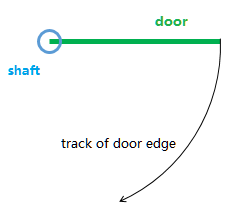
\includegraphics[height=5cm]{../pic/door.png}
				\caption{Typical scene when openning a door}
				\label{fig:door}
			\end{figure}
		
			Take a simple case for illustration, where a robot arm is trying to open the door shown in Fig(\ref{fig:door}). In traditional control strategy, the robot arm will move along the circle precisely. However, the actual track programmed by robot may be different due to noises like sensing errors. This is illustrated in Fig(\ref{fig:track}). In this case, the door will be broken by the robot arm or the robot arm will be pulled apart as the track of door edge will not change.
			 
			\begin{figure}[!ht]
				\centering
				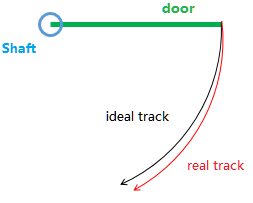
\includegraphics[height=5cm]{../pic/track.png}
				\caption{Real track of the robot arm}
				\label{fig:track}
			\end{figure}			
			
			A simple remedy is to add a spring in between like Fig(\ref{fig:spring}). In this way, errors are absorbed into the spring.
			
			\begin{figure}[!ht]
				\centering
				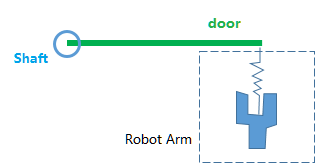
\includegraphics[height=5cm]{../pic/robot.png}
				\caption{Robot arm with spring}
				\label{fig:spring}
			\end{figure}	
		
			Also, friction is need to prevent endless vibration of the spring, which results in the 2nd-order ``Mass-Spring-Damper'' system shown in Fig(\ref{fig:arm}).
			
			\begin{figure}[!ht]
				\centering
				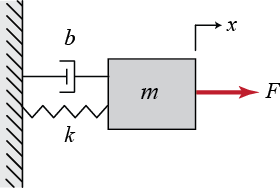
\includegraphics[height=5cm]{../pic/msd.png}
				\caption{Mass-Spring-Damper system}
				\label{fig:arm}
			\end{figure}
		
			Thus, the behaviour of this system can be described as follows:
			
			\begin{equation}
				M\frac{d^2 \textbf{x}}{d t^2} + b\frac{d \textbf{x}}{d t} + k \textbf{x} = \textbf{F} + \textbf{F}_{ext}\label{eq:newton}
			\end{equation}
			
			Impededance control is to modify $\textbf{F}$ according to measured position and difference to target track\cite{ref1}. This is usually done by changing the torque at joints. In this way, Eq(\ref{eq:newton}) can be re-formulated as
			
			\begin{equation}
				\textbf{F} = M\frac{d^2 \textbf{x}}{d t^2} + b\frac{d \textbf{x}}{d t} + k \textbf{x} - \textbf{F}_{ext}\label{eq:impedence}
			\end{equation}
			
			In order to provide suitable experience when interacting with human beings, the magnitude of \textbf{F} needs to be controlled exactly. Thus, a sensor measuring \textbf{F} is needed to provide feedback to controller. This is usually done by using a load cell.
		
	\end{itemize}

\begin{thebibliography}{16}  
	\bibitem{ref1}C. Ott, R. Mukherjee and Y. Nakamura, "Unified Impedance and Admittance Control," 2010 IEEE International Conference on Robotics and Automation, Anchorage, AK, 2010, pp. 554-561.
	doi: 10.1109/ROBOT.2010.5509861
\end{thebibliography}

\end{document}
